\chapter{Security}
\minitoc

\section{Lab Description}
\textit{The main objective of this week's assignment is to understand and analyze security models and protocols and furthermore implement a simple security protocol for task manager. As part of the assignment, you will study and develop a simple role based access control mechanism for tasks based on an authentication using ITU credentials. Moreover, you will also use one of the crypto algorithms to ensure security among all/some parts of communication.}

\section{Solution}

The handed-out project (before improvements) implements a simple security protocol. This protocol has a few short-commings. 1) The protocol is not secure against man-in-the-middle attacks and 2) how can the server trust the clients message is not a replay? Note \textit{The protocol implies that a successful decryption authenticates the sender!} \\

The challenges in the assignment includes how to implement an improved protocol that, among other things, allows a client and a server to exchange a shared secret key which then facilitates authenticated communication between them. How to improve the protocol to provide security against man-in-the-middle attacks and replays.  \\

The handed-out project uses shared private keys between participants i.e., private keys are known between [token server : server] and [token : server-client]. These keys are already distributed between the participants. The protocol, however, provides no means for the server to authenticate the client. Thus it is open to man-in-the-middle attacks and replays. A way to improve the protocol is to make the server able to authenticate the client, much like it is done in the Needham-Schroeder protocol.\\


In our solution, first the client sends a request to the authentication server (token server). The token server (upon authenticating the client with their shared secret key) sends back a encrypted response inside which is a ticket encrypted in the [token:server] private key, plus a session key for the communication between the client and the server. Note this is another insecure issue in the original protocol in that the authentication server (ITU server) have no means of authenticating the client. \\


\begin{lstlisting}
// from client to token server
{ credentials }K_tc
// from token service to client
{ {role, timestamp, identity, session key}K_ts, session key} 
\end{lstlisting}

The client is able to decrypt the response with the (already distributed) [token server : client] private key. The client now has a ticket plus the secret key (session key) to use for communicating with the server. The ticket is encrypted in the [token server : server] shared private key (so if the respons is intercepted its content is secure) and contains the [client : server] shared key (the session key) plus the clients identity, plus a timestamp and the clients role(note \textit{the server later uses the role to authenticate the client against an access rights table restricting access to it's resources}). \\ 

If this message (from the token-server to the client) is intercepted the encryption with the clients private key poses a challenge as do the ticket encrypted in the servers private key but, if the enemy manages to intercept and send the message to the server posing as the client, it is of no matter as the server then compares the identity in the ticket against the sender, and if they do not match the server denies access to its resources. Thus authenticating the client provides a protection against man-in-the-middle attacks.\\

Second, the client now in possesion of the session key, sends a 'authenticate' request to the server along with the ticket encrypted in the servers private key. The server decrypts the message and authenticates the client against the identity in the ticket. The session key has now been distributed between the server and client and will be used for communication between them. The ticket contains a timestamp used to timeout requests. \\ 

But first, the server sends a reply consisting of a message plus a nonce, encrypted with the [server : client] shared key (the session key). The purpose of the nonce is to provide proof to the server of message authenticity i.e., if the enemy intercepts and resends the message posing as the client, the server will be able to compare the nonces to authenticate the message.  

\begin{lstlisting}
// from client to server
authenticate, {role, timestamp, identity, session key}K_ts 
// from server to client
if(authenticated)
	yes, { nonce }K_sc // nonce, preventing replay
else
	no, {message}K_sc // nonce
\end{lstlisting}

When the server receives a new message from the client it should contain the nonce transformed by some agreed upon function (in this case simply the nonce - 1). By applying a transformation to the nonce the message/client effectively authenticates it's own identity to the server. Messages from the client must come in a predetermined order, the transformation of the nonce in each message in the communication-. The use of nonces prevents replay by numbering the messages in a way known to the server and client only. \\

If an enemy intercepts the message it will need to first deal with the session key after which it will still need to know which transformation of the nonce is the correct one in order to continue communicating with the server. \\

Only now do the client send a resource request to the server. the request message consists of a command plus the transformed nonce encrypted in the [client : server] shared key, plus the data on which to act, also encrypted in the shared key. \\

The server authenticates the message (against the transformed nonce) and the clients role against the access rights table. It replies by sending a message and yet a transformed nonce (the nonce could possibly be a new transformation of the same nonce?) on which further client-server communication is based.

%\pagebreak

\begin{lstlisting}
// from client to server
execute, {transformed nonce}K_sc, {data}K_sc
// from server to client
if(succesful execute)
	yes, {another nonce}K_sc
else
	no, {message}K_sc
\end{lstlisting}

In this, rather convoluted, way the server and client now has obtained a shared private key on which to communicate (more) securely. The protocol offers protection against man-in-the-middle attacks in several levels. The example uses nonces to authenticate the client and it provides the client identity, encrypted in the ticket, to the server again authenticating the client and the message as not a man-in-the-middle attack. The example still relies on a trusted third party, the principles involved still need to initially share secret keys. In the example the ITU server is the trusted source. \\
 
\begin{comment}
There's also still the possibility of a man-in-the-middle attack in where the message form the token server is send to the enemy, but ... 
\end{comment}

%\pagebreak

\section{Example run}

This is the console output....

\begin{figure}
\centering
\caption{example run}
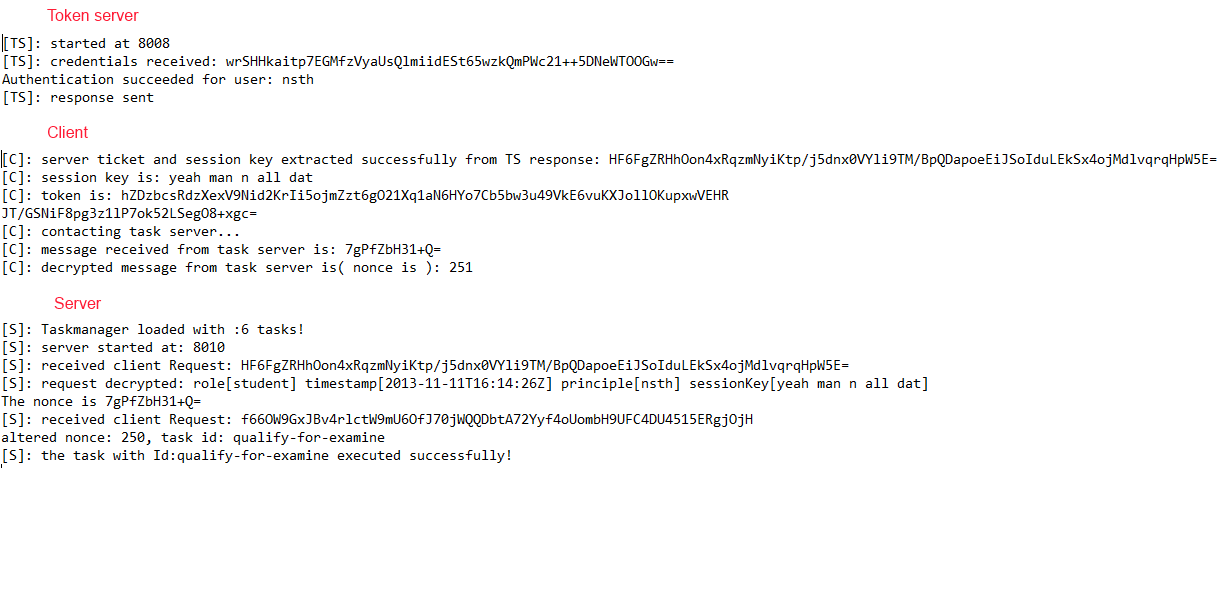
\includegraphics[scale=0.5]{images/security_run.png}
\end{figure}
\vspace{10pt}

\section{Reflection}

For a recap of Worst Case Assumptions an a definition of the enemy see the appendix.\\

The solution to security issues in distributed systems is to encrypt messages. All encryption algorithms are based on using a secret (called a key). Encryption algorithms use a key to obscure the content of messages (encrypt the message), and to decrypt the message. Encryption algorithms are based on one-way functions i.e., a function that converts an input to an output from which the input can not easily be deducted. \\ 

There are two types of keys and thus two types of encryption algorithms: \\

 \textbf{shared secret keys:} In which both the sender and the receiver knows the secret, note \textit{this is a solution for organizations which are able to distribute the secret key, secretely.}\\

\textbf{public/private key pairs:} In which a principle publishes a public key which can be used to encrypt messages. It doesn't matter if an enemy intercepts the key since only the coresponding private key can decrypt the message (idealy). Public/private algorithms (asymmetric algoritms) use trap-door functions. Trap-door functions are one-way functions that can be inversed by applying a key.  \\


In our example we used the JAVAX.CRYPTO package to encrypt end decrypt messages. We used the Data Encryption Standard (DES) algorithm but other algorithms can be used.\\

Cryptography plays three roles in implementing secure systems:\\

\textbf{Secrecy and Integrity:} Scenario1 (\textit{Secret communication by shared secret key }). A principle use a shared secret key to encrypt the messages and the receiving principle use the shared key to decrypt the messages(hence the name \textit{symmetric cryptography}). As long as the secret key is a secret secrecy is secure. There are two problems with this protocol: 1) How to share the secret key in the first place? and 2) how can the receiver trust the message is not a replay? Note \textit{This protocol implies that a successful decryption authenticates the sender!} \\

This is the scenario that the handed-out example (before we improved on it) closest resembles. There' no secret key between the server and client and the server can not be sure the messages from the client are not replays. \\

\textbf{Authentication:} Scenario2 (\textit{Authenticated communication with a server}). One way to provide authenticated communication is by involving a trusted source (say ... a server somewhere). The server hold secret keys for all participants. A principle requests the trusted server for access to a resource (say.. a server somewhere). The trusted source uses the principles key to authenticate the principle and then issues a response encrypted in the principles secret key (this is called a challenge. See below). The response contains a 'ticket' encrypted in the second principles secret key and a new secret key used for further communication between those two principles. \\ 

This is the protocol that closest resembles our finalized example. Note this protocol requires a trusted third party. A trusted third party is not always a possibility and the distribution of secret keys requires a secure channel which is not always possible either. \\

In this scenario a cryptographic challenge is used to eliminate the need for a principle to authenticate itself to the server. The reply sent back from the server is encrypted in the principles key, thus presenting a challenge that only the principle can overcome. This is a way of eliminating the need to keep sending a password over the network.\\

Scenario3 (\textit{Authenticated communication with public keys}). A principle makes a public/private key pair and makes the public key available. Anyone can encrypt a message using the public key but only the principle can decrypt those messages as he is the only one with the private key. \\

\begin{comment}
\textbf{Digital signatures:} Verification of the senders identity. Digital signatures uses a 'digest' of the message (a compressed form of the message). A digest is similar to a checksum. A digest function produces a digest of a message and the inverse function produces the message. The digest acts as a signature and accompanies the message.   
\end{comment}    
















 

  

\section{Conclusion}

Sending messages in distributed systems poses a security risk. The enemy can intercept messages, man-in-the-middle attack, and the resend the message posing as the client, replays. To protect against those we use encryption and carefully designed protocols. \\

Instead of authenticating by password we use a challenge. A challenge is an encryted message which can only be decrypted with the right key. Inside the encrypted message is a ticket, another challenge, encrypted in the server key. By adding the clients identity to the ticket a server can authenticate the sender of the message. By adding a sequence of nonces the server can authenticate subsequent messages from the client.\\

An enemy amy intercept the initial message from the client to the authentication/token server but will be unable to decrypt the message, and ticket inside. The enemy may send this message to the server anyway but the server can verify the sender's identity by comparing the identity inside the ticket to the sender. \\

An enemy may intercept messages from the client to the server and replay a message posing as the client but the sequence of nonces in the message enables the server to authenticate the message. If the enemey does not know the right nonce tranformation this is also a futile effort.\\

Though the security protocol in our example does provide protection against man-in-the-middle attacks and protection against replays it still assumes a trusted source. It assumes that the secret keys used for communication between principles and the trusted source are distributed safely. Eliminating the need for a trusted source is desirable but unatainable. \\

Even when principles share private keys there is a possibility of a man-in-the-middle attack. If the initial message from the client to the token server is intercepted the server will not be able to detect the attacker as it will be its identity inside the ticket. \\ 

This example used private keys. Using public/private keys would present a stronger encryption but suffer the same short-commings. \\

The nonce transformation function also need to be known by server and client. How can they share that secret securely?















